\subsection{Normals}
For each triangle $T=[p_1, p_2, p_3]$ of a triangle mesh, the normal is defined as
$$n(T) = \frac{(p_2 - p_1) \times (p_3 - p_1)}{||(p_2 - p_1) \times (p_3 - p_1)||}$$
The normal along each edge $E$ is halfway between the normals of two adjacent triangles $T_1$ and $T_2$
$$n(E) = \frac{n(T_1) + n(T_2)}{||n(T_1) + n(T_2)||}$$
The normal at vertex $V$ is obtained by averaging the normals of the $n$ adjacent triangles
$$n(V) = \frac{\sum_{i =1}^n \gamma_i n(T_i)}{||\sum_{i =1}^n \gamma_i n(T_i)||}$$
where $\gamma_i$ can be a constant value, equal to the triangle area or equal to the angle $\theta_i$ of $T_i$ at $V$ \cite{geometryprocessing}.
%%%%%%%%%%%%%%%%%%%%%%%%%%%%%%%%%%%%%%%%%%%%%%%%%%%%%%%%%%%%%%%%%

\subsection{Local averaging regions} \label{section:localaveraging}
Let us assume that a mesh is a piecewise linear approximation of a smooth surface.
A mesh can be constructed either as the limit of a family of smooth surfaces or as a linear approximation of an arbitrary surface. For each vertex of the neighbouring triangles (\textit{one-ring}), we can choose an associated surface patch over which the average of geometric properties will be computed.
Let $\mathcal{A}_{Barycenter}$ be the area formed using barycenters and $\mathcal{A}_{Voronoi}$ the one formed using \textit{Voronoi} cells. The general case is represented by a point that can be anywhere; let us denote this surface area $\mathcal{A}_M$.
\begin{figure}[!h]
    \centering
    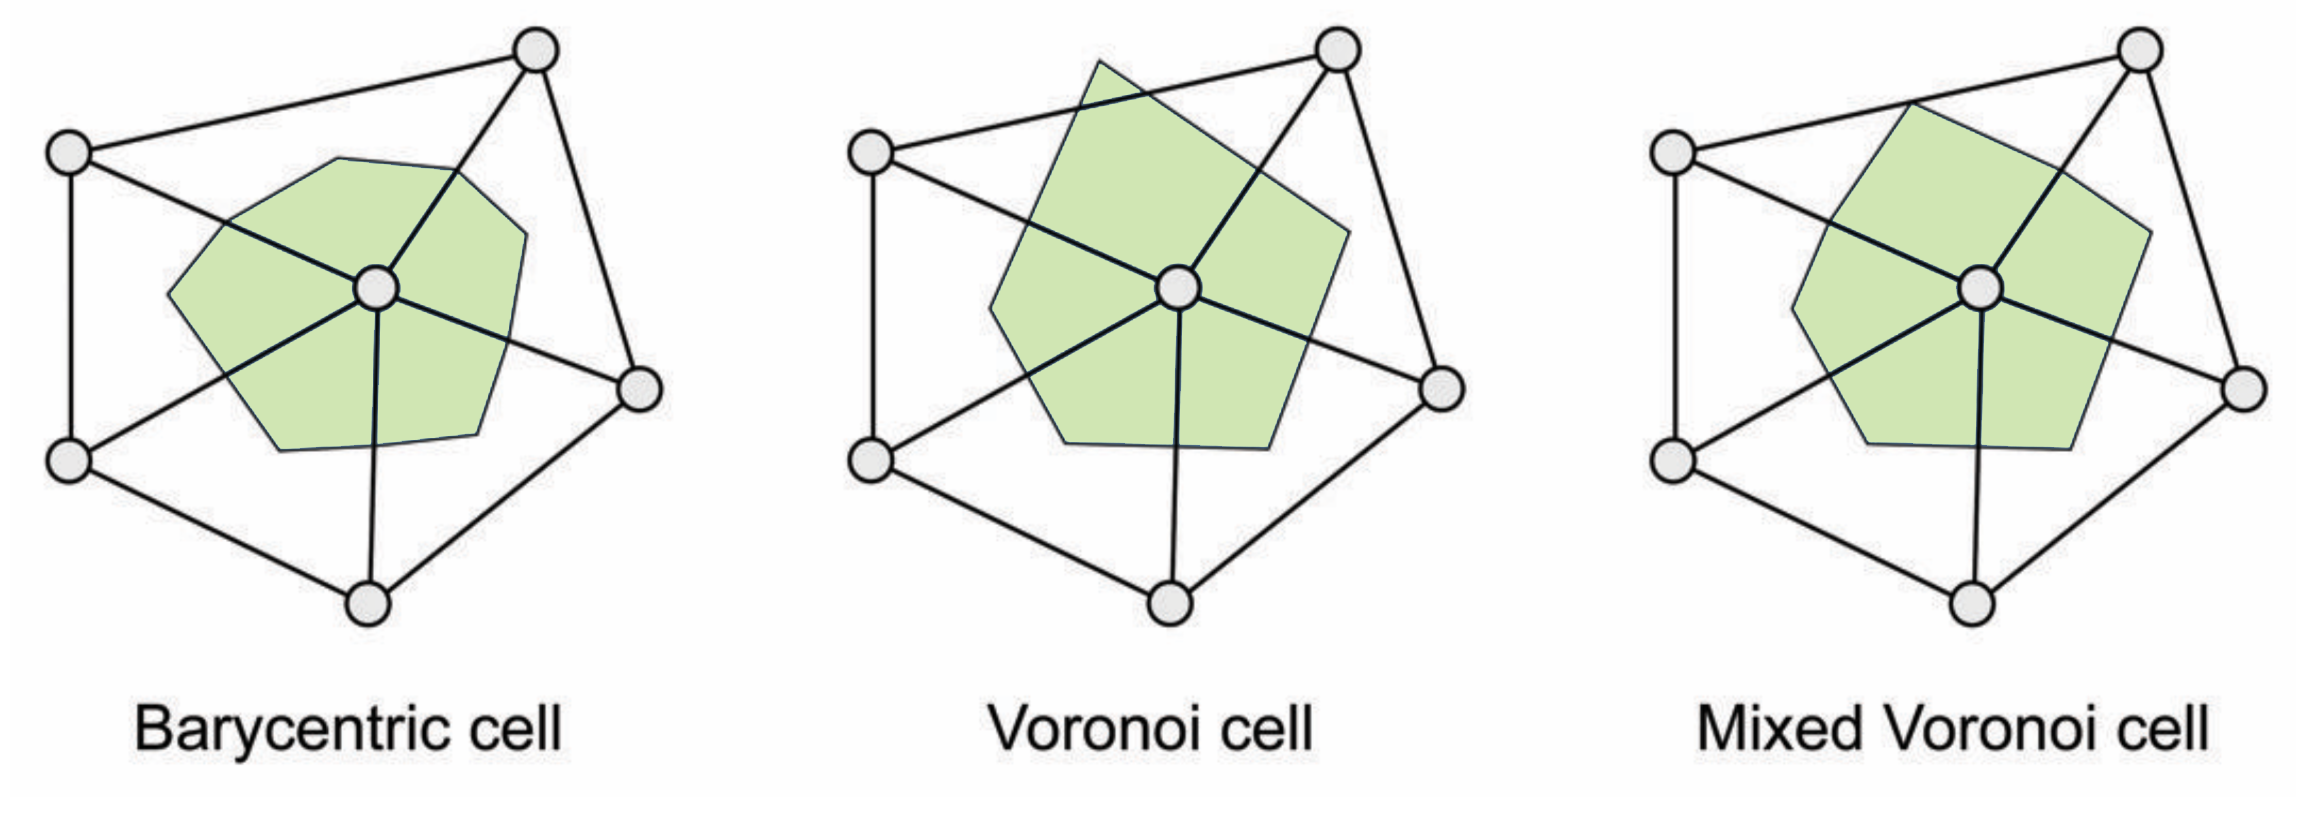
\includegraphics[scale=0.35]{images/localregions.png}
    \caption{Local averaging regions used for computing discrete differential operators associated with the center vertex of the one-ring neighborhood. $c_i$ corresponds to: the barycentre of the triangle in the Barycentric cell, the circumcenter of the triangle in the Voronoi cell. Let denominate $\theta$ the angle between $c_i$ and $c_{i+1}$. If $\theta < \frac{\pi}{2}$ then $c_i$ is on the circumcenter of triangle $[v_i, v, v_{i+1}]$, else $c_i$ is the midpoint of the edge $[v, v_{i+1}]$ in mixed Voronoi cell \cite{polygonmeshprocessing}.} \label{fig:localregions}
\end{figure}
\textit{Voronoi} cell of each vertex is an appropriate local region that provides a stable error bound.
The \textit{Voronoi} region for a point $P$ of a non-obtuse triangle $[P, Q, R]$ is expressed as $\frac{1}{8}(| PR|^2 cot \angle Q + |PQ |^2 cot \angle R)$. The sum of these areas for the whole \textit{1-ring neighborhood} gives the non-obtuse \textit{Voronoi} area for a vertex. The above expression for the \textit{Voronoi} finite-volume area does not hold in case of obtuse angles. Let us define a new surface area for each vertex denoted $\mathcal{A}_{Mixed}$. Essentially the idea is to use the circumcenter point for each non-obtuse triangle and to use the midpoint of the edge opposite to the obtuse angle in case of an obtuse triangle. (see Fig. \ref{fig:localregions} and pseudocode \ref{appendix:localaveraging}) \cite{meshlab}.

\subsection{Gaussian Curvature} \label{section:gaussian-curvature-intro}
The \textit{Gaussian curvature} $K$ is defined as the product of the principal curvatures:
$$K=k_1k_2$$
A basic interpretation would be to imagine the \textit{Gaussian curvature} as a logical \texttt{AND} since it checks whether there is a curvature along both directions.
The curvature of a surface is characterized by the principal curvatures \cite{WEBSITE:gaussiancurvaturedirty}.
%---------
\begin{figure}[!h]
  \centering
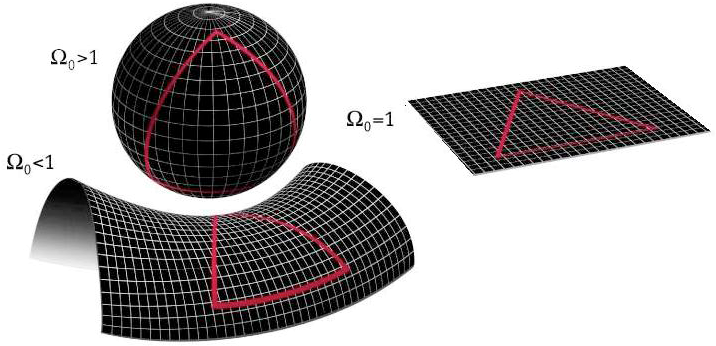
\includegraphics[scale=0.5]{images/gaussian_curvature_examples.png}
\caption{Positive curvature, negative curvature and zero curvature.}\label{fig:curvature-gaussian}
\end{figure}
Surfaces that have a zero Gaussian curvature are called \textit{developable surfaces} because they can be flattened out into the plane without any stretching. \textit{Gaussian curvature} is zero inside each mesh triangle and the same along edges since it can be flattened symmetrically into the plane. Consequently the \textit{Gaussian curvature} is concentrated at vertices of a triangle and it is defined as the \textit{angle defect}
$$K(V) = 2 \pi - \sum_{i=1}^n \theta_i$$
where $\theta_i$ is the angles of the triangle $T_i$ adjacent to the vertex $V$ at $V$. This should be seen as the integral of the Gaussian curvature over a certain region $S(V)$ around $V$, where these $S(V)$ form a partition of the surface of the entire mesh.
$$ K(V) = \int_{S(V)} KdA  $$
\textit{Negative curvature} can be recognized by the fact that external directions curve in opposite directions, \textit{zero curvature} has one external direction that has zero curvature, \textit{positive curvature} has external directions that curve in the same direction (Fig. \ref{fig:curvature-gaussian}).
The \textit{Theorema Egregium}, discovered by C.F. Gauss in 1827, states that the \textit{Gaussian curvature} is an intrinsic property of the surface that does not depend on the space, despite the fact that it is defined as the product of the principal curvatures (whose value depends on how the surface is immersed in the space).
We can then notice that triangle angles add up to less than $180 \degree$ in negative curvature, exactly $180 \degree$ in zero curvature, and more than $180 \degree$ in positive curvature \cite{geometryprocessing}.
%%%%%%%%%%%%%%%%%%%%%%%%%%%%%%%%%%%%%%%%%%%%%%%%%%%%%%%%%%%%%%%%%

\subsection{Mean Curvature}
The \textit{mean curvature} $H$ is defined as the arithmetic mean of principal curvatures $$H = \frac{k_1 + k_2}{2}$$  A basic interpretation would be to imagine the \textit{mean curvature} as a logical \texttt{OR} since it checks if there is a curvature along at least one direction \cite{WEBSITE:gaussiancurvaturedirty}.
The \textit{mean curvature} inside each mesh triangle is zero, but it does not vanish at edges. The \textit{mean curvature} associated with an edge is defined as $H(E) = \parallel E \parallel {\theta}_E/2$, where ${\theta}_E$ is the signed
angle between the normals of adjacent triangles (see Fig. \ref{fig:mean-curvature}).

\begin{figure}[!h]
  \centering
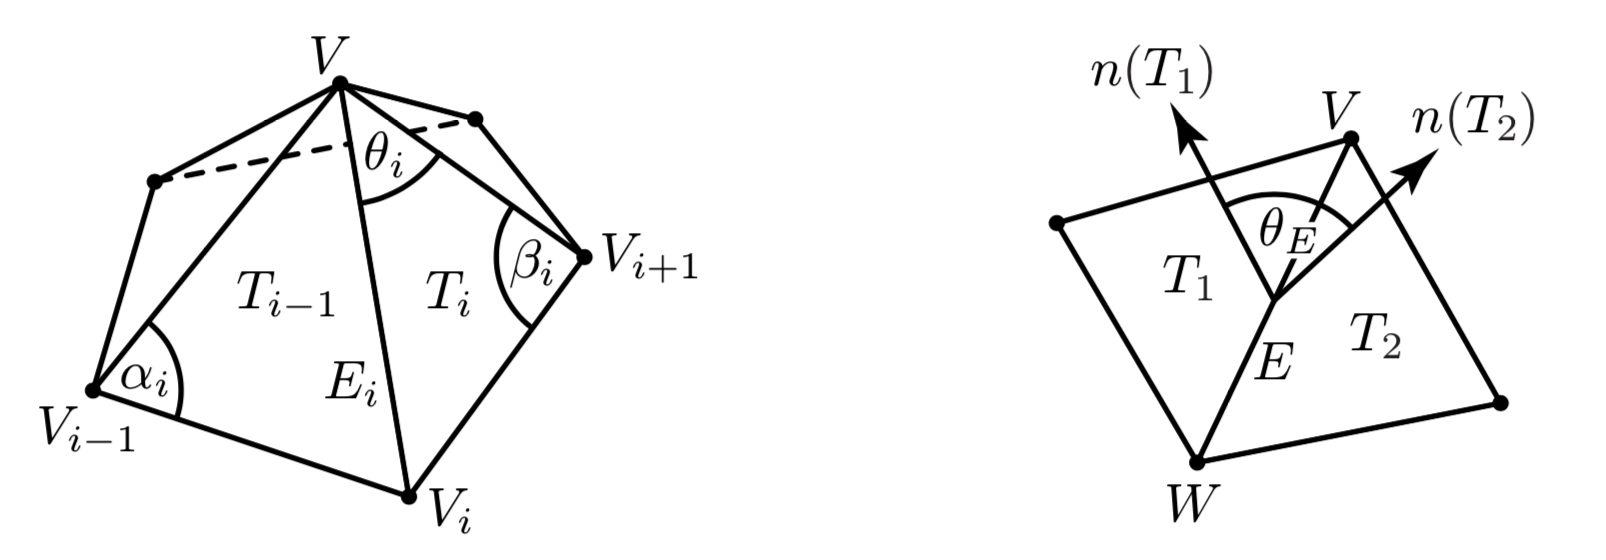
\includegraphics[width=11.5cm]{images/mean_curvature_paper.png}
\caption{A vertex $V$ with its neighbouring vertices $V_i$ and adjacent triangles $T_i$. Angles opposite the edge $E_i$ are denoted by $\alpha_i$ and $\beta_i$. The
angle between the normals of adjacent triangles $T_1$ and $T_2$ with positive or negative sign is denoted as ${\theta}_E$ \cite{geometryprocessing}}\label{fig:mean-curvature}.
\end{figure}
Let us think of an edge as a cylindrical patch $C(E)$ with a radius $r$ that touches the planes defined by adjacent triangles. The \textit{mean curvature} at any point of the cylindrical patch is defined as $1/(2r)$ and the area of $C(E)$ is $r||E||\theta_E$
$$H(E) = \int_{C(E)} HdA$$
The \textit{mean curvature} at the vertex $V$ is defined as $$H(V) = \frac{1}{2} \sum_{i=1}^n H(E_i)$$ Averaging the mean curvatures of its adjacent edges guarantee that \textit{mean curvature} of an edge is divided uniformly to both end points. $H(E)$ and $H(V)$ should be seen as integral curvature values associated to regions $S(E)$ and $S(V)$ \cite{geometryprocessing}.

%%%%%%%%%%%%%%%%%%%%%%%%%%%%%%%%%%%%%%%%%%%%%%%%%%%%%%%%%%%%%%%%%

\subsection{Mean Curvature Vector}
Let $\bm{H} = H n$ be the surface normal vector scaled by the \textit{mean curvature}. We can integrate it over the $C(E)$ to derive the discrete mean curvature vector associated to the mesh edge $E=[V, W]$:
$$ \bm{H}(E) = \int_{C(E)} \bm{H}dA = \frac{1}{2} (V-W) \times (n(T_1) - n(T_2))$$
The length of $H(E)$ gives the edge mean curvature $H(E) = ||\bm{H}(E) || = ||E|| sin(\theta_E/2)$. The discrete mean curvature vector associated to $V$ can be obtained averaging $\bm{H}(E)$ over the edges adjacent to a vertex $V$
$$\bm{H}(V) = \frac{1}{2} \sum_{i=1}^{n} \bm{H}(E_i) = \frac{1}{4}\sum_{i=1}^n (\cot \alpha_i + \cot \beta_i)(V - V_i)$$
where $\alpha_i$ and $\beta_i$ are angles opposite to $E_i$ (see Fig. \ref{fig:mean-curvature}) \cite{geometryprocessing}.
